\documentclass[fleqn]{article}
\usepackage[utf8]{inputenc}

\title{Compte rendu\\ Projet de Calcul Scientifique Numérique} 
\author{Belpois Vincent \\ Chomette Hugo}
\date{}
\usepackage[fleqn]{mathtools}
\usepackage{amssymb}
\usepackage{enumitem}
\usepackage{amsfonts}
\usepackage{amsmath}
\usepackage{geometry}
\usepackage{graphicx}
\usepackage{xcolor}
\usepackage{esint}          % various fancy integral symbols
\usepackage{upgreek}
\usepackage{parskip}
\usepackage[b]{esvect}      %For better vectors
\usepackage{float}
\usepackage{tikz}


\usepackage{pdflscape}
\usepackage{hyperref}
\hypersetup{
    colorlinks,
    citecolor=black,
    filecolor=black,
    linkcolor=black,
    urlcolor=black
}


\geometry{hmargin=2.5cm,vmargin=2cm}

\usepackage{sectsty}
%\sectionfont{\color{red}}
%\subsectionfont{\color{red}}
%\renewcommand{\thesection}{\color{red} \Roman{section}\color{black} } 
%\renewcommand{\thesubsection}{{ \indent \arabic{subsection}) }}
%\renewcommand{\thesubsubsection}{\indent \indent \alph{subsubsection}.} 
\renewcommand*\contentsname{Table des matières}

\renewcommand{\epsilon}{\varepsilon} 
\renewcommand{\phi}{\varphi} 
\newcommand{\dd}{\text{d}}

\let\vect\overrightarrow
\let\mc\mathcal




\setlist[1]{noitemsep}



\begin{document}
\maketitle
\newpage

\tableofcontents
\newpage

\section{Présentation du problème}
\subsection{Le problème}
On modélise un thermocouple par une sphère uniforme de rayon $a$. Cette sphère, initialement à la température $T_0$, échange convectivement avec le milieu extérieur, à la température $T_\infty$, selon la loi $\phi = h(\theta) ( T - T_\infty)$. 
\begin{figure}[H]
    \centering
    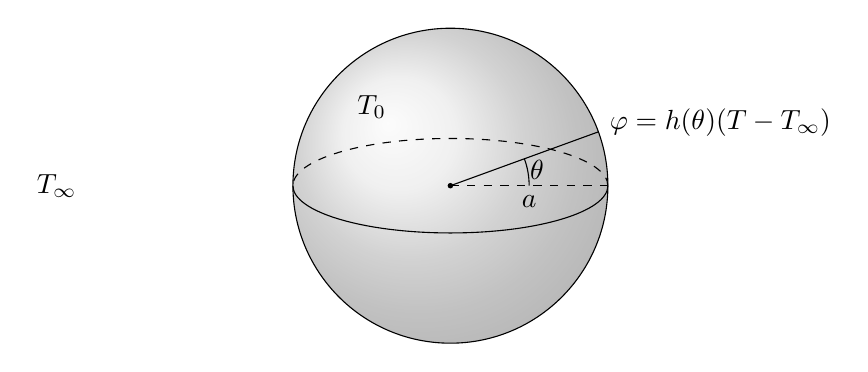
\begin{tikzpicture}
        \shade[ball color = gray!40, opacity = 0.4] (0,0) circle (2cm);
        \draw (0,0) circle (2cm);
        \draw (-2,0) arc (180:360:2 and 0.6);
        \draw[dashed] (2,0) arc (0:180:2 and 0.6);
        \fill[fill=black] (0,0) circle (1pt);
        \draw[dashed] (0,0 ) -- node[below]{$a$} (2,0);
        \draw (0,0) -- ({2*cos(20)},{2*sin(20)});
        \draw (1,0) arc (0:20:1);
        \node at (1.1,0.2) {$\theta$};
        \node at (1.9,0.8) [right]{$\phi = h(\theta) ( T - T_\infty)$};
        \node at (-5, 0) {$T_\infty$};
        \node at (-1,1) {$T_0$};
    \end{tikzpicture}
    \caption{Schéma du Thermocouple}
\end{figure}


On cherche alors à étudier la réponse de ce thermocouple au cours du temps. Pour cela, on s'impose l'utilisation de la méthode des différences finies


\subsection{Interprétation des coéficients}
La fonction $h(\theta)$ décrit la dépendance de la convection avec l'angle $\theta$ entre la normale à la surface de la sphère et la direction de l'échange thermique. Plus précisément, la quantité de chaleur échangée par convection entre la sphère et le milieu extérieur est proportionnelle à la différence de température entre la sphère et le milieu extérieur, multipliée par $h(\theta)$.

La forme de la fonction $h(\theta) = K (1 + \cos(\theta))$ indique que l'échange de chaleur par convection est maximale lorsque la normale à la surface de la sphère est parallèle à la direction de l'échange thermique et dans le me sens que celui-ci, c'est-à-dire lorsque $\theta = 0^\circ$. Dans ces cas, $h(\theta) = K (1 + 1) = 2K$. L'échange de chaleur par convection est minimale lorsque la normale à la surface de la sphère est dans le sens opposé à celui de l'échange thermique, c'est-à-dire lorsque $\theta = 180^\circ$. Dans ce cas, $h(\theta) = K (1 - 1) = 0$.

La constante $K$ détermine l'intensité de l'échange de chaleur par convection pour un angle $\theta$ donné. Plus $K$ est grand, plus l'échange de chaleur par convection est important. $K$ est alors exprimé en $W.m^{-2}.K^{-1}$, tout comme $h(\theta)$.

\subsection{Mise en équation du problème}
Ce problème revient alors a résoudre l'équation de la chaleur en 3 dimmensions et au cours du temps.
De manière générale, l'équation de la chaleur s'écrit de la manière suivante.
\begin{equation}
    \rho C_p \left(  \frac{ \partial T}{\partial t} + u \cdot \nabla T \right) = \nabla \cdot ( \lambda  \nabla T) + s
\end{equation}

Dans notre cas, cette équation peut être simplifiée. On a premièrement $u = 0$ car la sphère n'est pas en mouvement. De plus, lambda est constant, on a donc par linéaritée du gradiant $\nabla ( \lambda \nabla T ) = \lambda \nabla^2 T$. Enfin, le thermocouple n'étant traversé par aucun courant électrique, aucune chaleur n'est produit en sont sein et don cle terme de source $s$ est nul.

L'équation de la chaleur devient alors :
\begin{equation}
    \rho C_p   \frac{ \partial T}{\partial t} = \lambda\nabla^2 T
    \label{equation de la chaleur}
\end{equation}


\section{Choix du système de coordonnées et du maillage}
\subsection{Comparaison des systèmes de coordonnées cartésiennes et sphériques}
\subsubsection{Coordonnées cartésiennes}
Le système de coordonnées cartésiennes a l'avantage d'utiliser un repère orthonormé. L'expression des opérateurs tels que le laplacien est donc simple et les équation sont alors simplifiées. Cependant, si le maillage n'est pas régulier selon les trois axes du système de coordonnées cartésiennes, l'expression du pas est alors plus complexe.

\begin{figure}[H]
    \centering
    \textbf{AJOUTER PETIT REPERE CARTESIEN}
\end{figure}

\subsubsection{Coordonnées sphériques}
Le problème décrivant une sphère, le seul système de coordonnées qui peut être intéressant à utiliser est le système de coordonnées sphériques. Ce système de coordonnées est aussi constitué de trois axes orthonormés:$\vv{e_r}, \vv{e_\theta}, \vv{e_\phi}$ . On utilisera alors pour décrire la position d'un point un triplet de coordonées $(r, \theta, \phi)$. 

\begin{figure}[H]
    \centering
    \textbf{AJOUTER PETIT REPERE SPHERIQUE}
\end{figure}


Pour passer des coordonées cartésiennes aux coordonées sphériques on utilise les équtions suivantes :
\begin{equation}
    \begin{cases}
        r = \sqrt{x^2 + y^2 + z^2} \\
        \theta = \arccos \left( \frac{z}{r} \right)\\
        \phi = \arctan \left( \frac{y}{x} \right)
    \end{cases}
\end{equation}

De la même manière, pour passer des coordonnées sphériques aux coordonnées cartésiennes on utilise les équations suivantes :
\begin{equation}
    \begin{cases}
        x&=r \sin \theta \cos \varphi \\y&=r \sin \theta \sin \varphi \\z&=r \cos \theta 
    \end{cases}
\end{equation}

\subsection{Réécriture des équations adaptée au nouveau système de coordonnées}
 
L'équation de la chaleur Eq.\eqref{equation de la chaleur} utlise l'opérateur laplacien ($\Delta = \nabla^2$). Cet opérateur s'écrit en coordonnées cartésiennes :

\begin{equation}
    \Delta f = {\frac {\partial ^{2}f }{\partial x^{2}}}+{\frac {\partial ^{2}f }{\partial y^{2}}}+{\frac {\partial ^{2}f }{\partial z^{2}}}
\end{equation}

En coordonnées sphérique, cet opératreur s'écrit alors :
\begin{equation}
     \Delta f={\frac {\partial ^{2}f}{\partial r^{2}}}+{\frac {2}{r}}{\frac {\partial f}{\partial r}}+{\frac {1}{r^{2}}}{\frac {\partial ^{2}f}{\partial \theta ^{2}}}+{\frac {1}{r^{2}\tan \theta }}{\frac {\partial f}{\partial \theta }}+{\frac {1}{r^{2}\sin ^{2}\theta }}{\frac {\partial ^{2}f}{\partial \varphi ^{2}}}
\end{equation}

L'équation de la chaleur Eq.\eqref{equation de la chaleur} s'écrit alors :
\begin{equation}
    \rho C_p \frac{ \partial T}{\partial t}  = \lambda \left( 
    {\frac {\partial ^{2}T}{\partial r^{2}}}+{\frac {2}{r}}{\frac {\partial T}{\partial r}}+{\frac {1}{r^{2}}}{\frac {\partial ^{2}T}{\partial \theta ^{2}}}+{\frac {1}{r^{2}\tan \theta }}{\frac {\partial T}{\partial \theta }}+{\frac {1}{r^{2}\sin ^{2}\theta }}{\frac {\partial ^{2}T}{\partial \varphi ^{2}}} \right)      
\end{equation}
Dans la suite du problème on utilisera la constante $\alpha = \frac{\lambda}{\rho C_p}$ afin de simplifier l'écriture de l'équation ci-audessus.

\subsection{Maillage de la sphère}

\section{Discrétisation du problème} 
\subsection{Discrétisation de l'équation de la chaleur}
\subsection{Discrétisation des condition aux limites}



\newpage
\section{Simulation Python} 
Petite introduction sur pourquoi on a utiliser python pour faire cette simulation
\subsection{Structure du code}
\subsection{Implémentation du maillage}
\subsubsection{Maillage et simulation}
explication du type mesh

explication de la list de meshes qui est alors une simulation
\subsubsection{Implémentation des maillages et des simulations}
\subsection{Implémentation des équations}
\subsection{Simulations}
\subsubsection{Choix des valeurs des paramètre}
Choix des pas, des dimensions, de Delta t, du temps de simulation
\subsubsection{Test de l'influence de certains paramètres}
\subsubsection{Simulations}

\newpage
\section{Conclusion}
Conclure sur la méthode utilisé, l'implémentation, la convaincance des résultats.

Finir sur ce que cela nous a apris, la facilitée d'implémenter vs la difficultée à discrétiser le probblème et choisir la valeur des paramètres

\end{document}